The \textit{Repository Management} module is responsible for management and cataloging of
algorithms and test data to be used in the benchmarking tests.

\subsection{Domain Model}
The domain model for the Repository Management module is shown in Figure \ref{fig:repoManDomain}
\begin{figure}[H]
  \begin{center}
  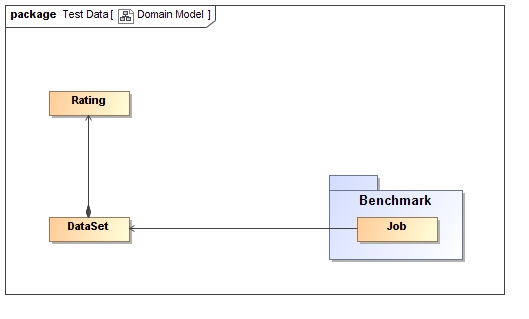
\includegraphics[scale=0.5]{../Diagrams and Charts/Test Data/Domain Model.jpg}  
  \caption{Repository Management Domain Model}
  \end{center}
  \label{fig:repoManDomain}
\end{figure}
\clearpage
\subsection{Scope}
The scope for the Repository Management module is shown in Figure \ref{fig:repoManScope}
\begin{figure}[H]
  \begin{center}
  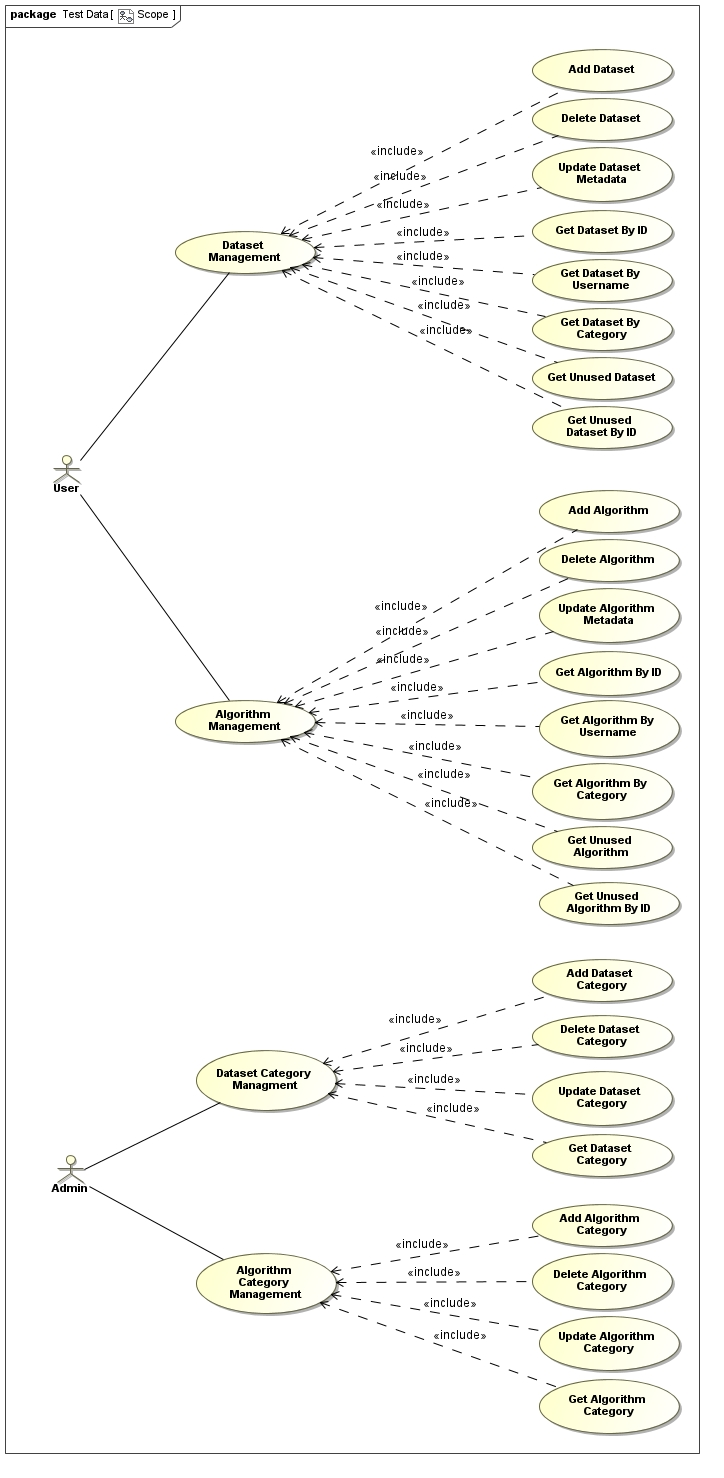
\includegraphics[scale=0.34]{../Diagrams and Charts/Test Data/Scope.jpg}
  \caption{Scope of Categories}
  \end{center}
  \label{fig:repoManScope}
\end{figure}

\subsection{Dataset Management}

\subsubsection {Users will be able to add a dataset}
The service contract for adding a dataset is shown in Figure \ref{fig:addDatasetService}
\begin{figure}[H]
  \begin{center}
  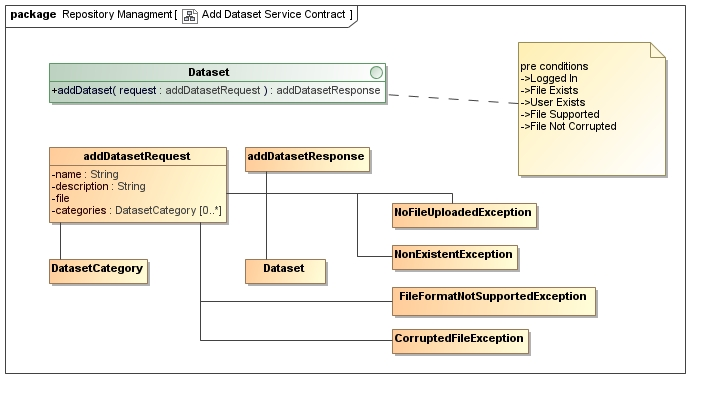
\includegraphics[scale=0.6]{../Diagrams and Charts/Test Data/Add Dataset Service Contract.jpg}
  \caption{Add Dataset Service Contract}
  \end{center}
  \label{fig:addDatasetService}
\end{figure}

\subsubsection {Users will be able to delete a dataset}
\subsubsection {Users will be able to update a dataset}
\subsubsection {Users will be able to get a dataset by ID}
\subsubsection {Users will be able to get a dataset by name}
\subsubsection {Users will be able to get a dataset by category}
\subsubsection {Users will be able to get all unused datasets}
\subsubsection {Users will be able to get an unused dataset by ID}

\subsection{Algorithm Management}

\subsubsection {Users will be able to add an algorithm}
\paragraph{Service Contract}\\
The service contract for adding an algorithm is shown in Figure \ref{fig:addAlgorithmService}

\begin{figure}[H]
  \begin{center}
  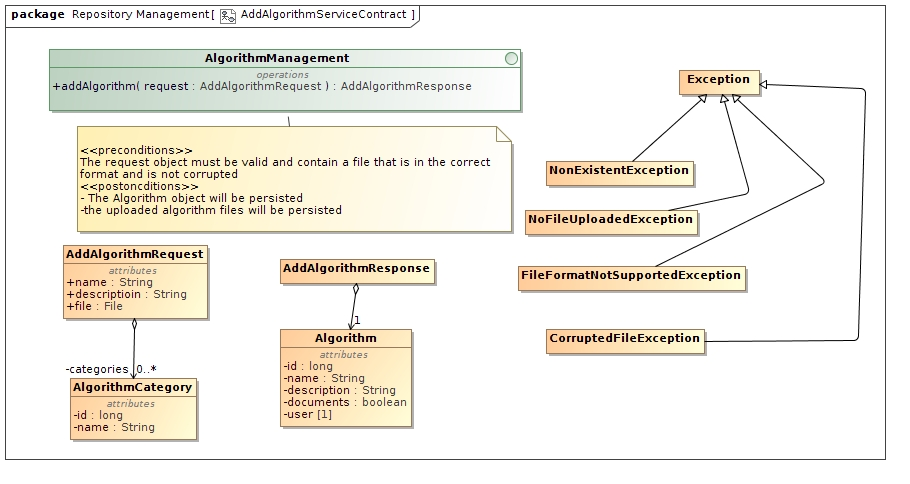
\includegraphics[scale=0.5]{../Diagrams and Charts/Test Data/AddAlgorithmServiceContract.jpg}
  \caption{Add Algorithm Service Contract}
  \label{fig:addAlgorithmService}
  \end{center}  
 \end{figure}

 The service will add the Algorithm meta data as well as the store the
 actual Algorithm files to a database.\\\\
 The service will be refused if:\\
	 \begin{itemize}
	 	\item The request object does not have a valid structure.	 	
	 	\item The request object does not contain a file.
	 	\item The file is not in an acceptable format
	 	\item The file is corrupted
	 \end{itemize}
In each case the appropriate exception will be thrown.
\subsubsection {Users will be able to delete an algorithm}
\subsubsection {Users will be able to update an algorithm}
\subsubsection {Users will be able to get an algorithm by ID}
\subsubsection {Users will be able to get an algorithm by name}
\subsubsection {Users will be able to get an algorithm by category}
\subsubsection {Users will be able to get all unused algorithms}
\subsubsection {Users will be able to get an unused algorithm by ID}

\subsection{Dataset Category Management}

\subsubsection {Admin will be able to add a dataset category}
The service contract for adding a dataset category is shown in Figure \ref{fig:addDatasetCatService}
\begin{figure}[H]
  \begin{center}
  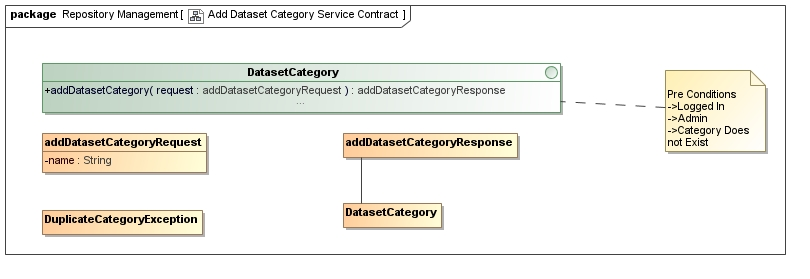
\includegraphics[scale=0.6]{../Diagrams and Charts/Test Data/Add Dataset Category Service Contract.jpg}
  \caption{Add Dataset Category Service Contract}
  \end{center}
  \label{fig:addDatasetCatService}
\end{figure}

The pre-conditions
\begin{itemize}
  \item User needs to be an admin
  \item All details of the new dataset category need to be valid
  \item Category must not exist
\end{itemize}

The post-conditions
\begin{itemize}
  \item Category is created succesfully
\end{itemize}

\subsubsection {Admin will be able to delete a dataset category}

The service contract for deleting a dataset category is shown in Figure \ref{fig:deleteDatasetCatService}
\begin{figure}[H]
  \begin{center}
  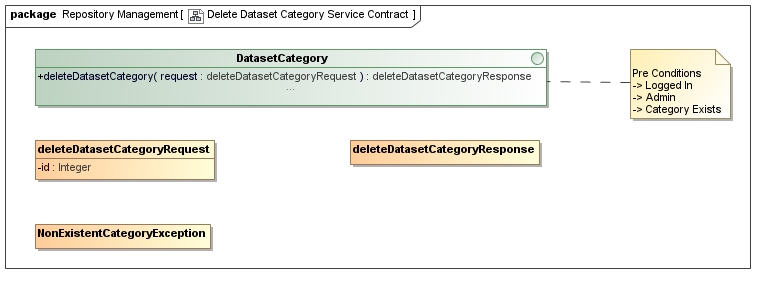
\includegraphics[scale=0.6]{../Diagrams and Charts/Test Data/Delete Dataset Category Service Contract.jpg}
  \caption{Delete Dataset Category Service Contract}
  \end{center}
  \label{fig:deleteDatasetCatService}
\end{figure}

The pre-conditions
\begin{itemize}
  \item User needs to be an admin
  \item Category must exist
\end{itemize}

The post-conditions
\begin{itemize}
  \item Category is deleted succesfully
\end{itemize}

\subsubsection {Admin will be able to update a dataset category}

The service contract for updating a dataset category is shown in Figure \ref{fig:updateDatasetCatService}
\begin{figure}[H]
  \begin{center}
  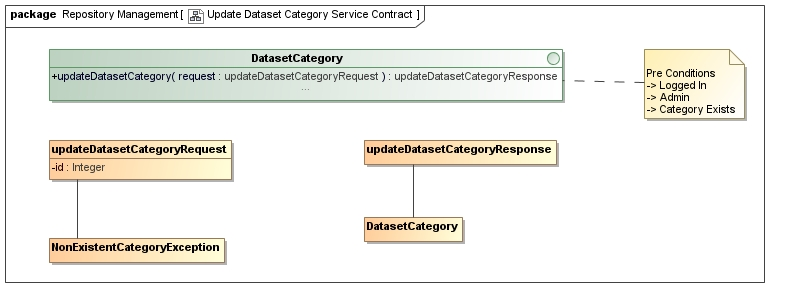
\includegraphics[scale=0.6]{../Diagrams and Charts/Test Data/Update Dataset Category Service Contract.jpg}
  \caption{Update Dataset Category Service Contract}
  \end{center}
  \label{fig:updateDatasetCatService}
\end{figure}


The pre-conditions
\begin{itemize}
  \item User needs to be an admin
  \item Category must exist
  \item New details must be valid
\end{itemize}

The post-conditions
\begin{itemize}
  \item Category is updated succesfully
\end{itemize}
\subsubsection {Admin will be able to get a dataset category}

The service contract for getting a dataset category is shown in Figure \ref{fig:getDatasetCatService}
\begin{figure}[H]
  \begin{center}
  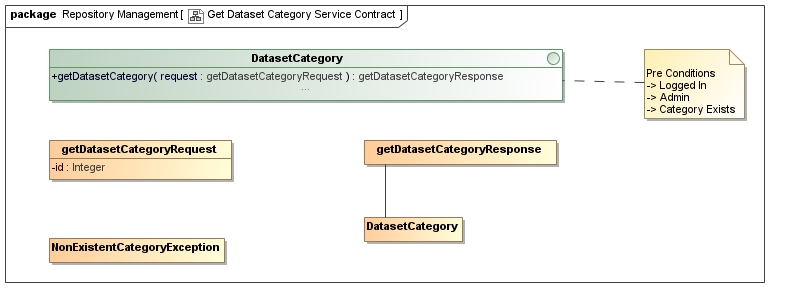
\includegraphics[scale=0.6]{../Diagrams and Charts/Test Data/Get Dataset Category Service Contract.jpg}
  \caption{Get Dataset Category Service Contract}
  \end{center}
  \label{fig:getDatasetCatService}
\end{figure}

The pre-conditions
\begin{itemize}
  \item User needs to be an admin
  \item Category must exist
\end{itemize}

The post-conditions
\begin{itemize}
  \item Category is gotten succesfully
\end{itemize}

\subsection{Algorithm Category Management}

\subsubsection {Admin will be able to add a algorithm category}
\subsubsection {Admin will be able to delete a algorithm category}
\subsubsection {Admin will be able to update a algorithm category}
\subsubsection {Admin will be able to get a algorithm category}







